\documentclass{article}
%http://tex.stackexchange.com/a/196456/7712
\usepackage{tikz,etoolbox}
\usetikzlibrary{calc}

\makeatletter
\newcount\@eledtikzline
\@eledtikzline=1
\xdef\@eledtikzlines{}

\newcommand{\beledtikzline}{%
  \the\@eledtikzline%
}

\def\lines{1,2,3}

\begin{document}

  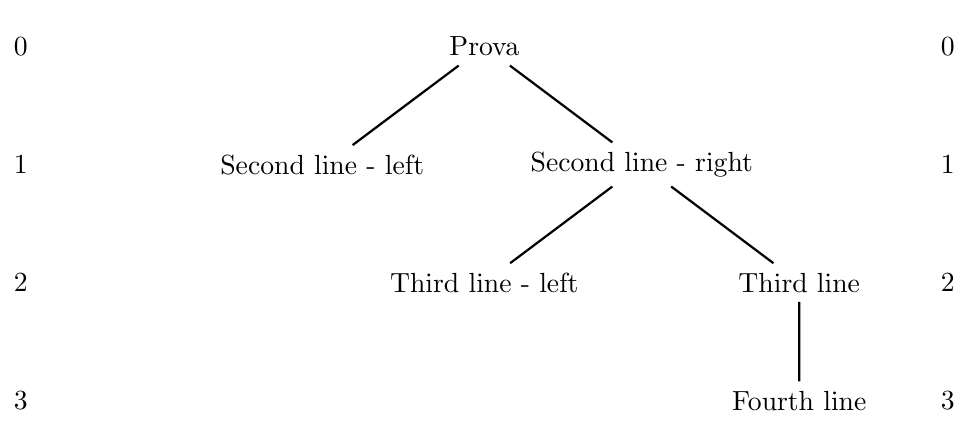
\begin{tikzpicture}[sibling distance=4cm,
                      edge from parent/.style={draw,thick}]
   \node(A){Prova}
        child {node(B)[align=left] {Second line - left } }
        child {node[align=right] {Second line - right}
            child {node (C)[align=left] { Third line - left}}
            child {node {Third line }
              child {node(D){Fourth line}}
              }
        };

  
  \foreach \Node in {A,B,C,D} {%\y1=y-coord of the node
    \path let \p1=($ (\Node) $) in node at (0,\y1)[inner sep=0,outer sep=0,text width=\textwidth-\parindent]{
    \llap{\the\@eledtikzline}\hfill\rlap{\the\@eledtikzline}};
    \global\advance\@eledtikzline by1
  }
\end{tikzpicture}




\leavevmode\llap{\the\@eledtikzline}\hfill main text\hfill \rlap{\the\@eledtikzline}
    \global\advance\@eledtikzline by1
    
\leavevmode\llap{\the\@eledtikzline}\hfill main text\hfill \rlap{\the\@eledtikzline}

\end{document}